% =====================================================================
% CHAPITRE 1 : RISQUE CYBER, RESILIENCE NUMERIQUE ET BESOIN DE CAPITAL.
%
% CE CHAPITRE SUIT LE PLAN ARRETE PAR KELIAN. Cinq sections, de la definition du risque a la
% problematique, sur le modele progressif du chapitre 1 de F. Dountio (ENSAE, 2026).
%
% CE QU'IL ABSORBE, ET C'EST LA DECISION DE STRUCTURE LA PLUS LOURDE DU FICHIER. Le plan met
% DORA en section 4 et la problematique en 5.3, or ces deux contenus vivent aujourd'hui dans
% 04_cadre_reglementaire.tex et 02_introduction.tex. SI CE CHAPITRE EST RETENU :
%   - 02_introduction.tex doit disparaitre ou se reduire a ce que 2b.5.3 ne reprend pas. Sa
%     section LUCY (sec:lucy) est reprise ici en section 3 et NE DOIT PAS figurer deux fois ;
%   - 04_cadre_reglementaire.tex doit se reduire a la seule articulation avec Solvabilite II,
%     le cadre DORA lui-meme passant ici. Son label chap:reglementaire doit survivre, cinq
%     chapitres le citent.
% Ne pas compiler le document avec ce chapitre ET les deux autres en l'etat : le lecteur lirait
% deux fois la meme lecture de marche et deux fois les cinq piliers.
%
% LES TROIS SOURCES DE CONTEXTE ET LEUR STATUT. Les valeurs 2026 de la cartographie France
% Assureurs, du barometre CESIN et de l'etude LUCY sont TRANSCRITES dans config.py sous
% CARTO_FA_2026, CESIN_2026 et LUCY_2026, au statut de CITATION EXTERNE NON RECALCULABLE. Le
% depot ne detient aucune de ces donnees d'origine : il ne peut que verifier la fidelite de la
% recopie, ce que font les scripts 63 (LUCY) et 103 (cartographie et barometre). Aucune n'entre
% dans une calibration et aucune ne porte un montant de capital. NE PAS ecrire une valeur de ces
% sources directement ici : elle echapperait au harnais, ce qui est la classe de defaut qui a
% produit les queues Bale et le Hill a 1,42.
%
% LES FIGURES SONT EXTRAITES DES RAPPORTS, comme les trois figures LUCY, et vivent dans
% memoire_cascade/figures_externes/, exception declaree du projet. Son README doit etre complete
% pour chaque figure ajoutee : provenance, page, recadrage. L'AUTORISATION DE REPRODUCTION EST
% ACQUISE POUR TOUTES : accordee par Hugo Rapior le 17 septembre pour les figures LUCY, puis
% etendue par lui le 19 septembre a la cartographie France Assureurs, au barometre CESIN et a la
% carte Avast. Ne pas rouvrir.
%
% AUCUNE FIGURE EN PLEINE PAGE. La macro de figure cle est interdite depuis le 15 septembre.
% Figures en ligne, 5 a 9 cm imprimes.
% =====================================================================

\chapter{Risque cyber, résilience numérique et besoin de capital}
\label{chap:cadre-cyber-dora}

\begin{cle}
\textbf{Ce que ce chapitre établit.} Le risque cyber n'est pas un risque de plus dans un
portefeuille. Sa sinistralité est portée par un petit nombre d'événements, ses causes se
propagent d'une organisation à l'autre par les prestataires qu'elles partagent, et le marché
qui l'assure ne dispose pas de la profondeur d'historique nécessaire pour en estimer la queue.
Ces trois traits commandent respectivement le choix d'une modélisation par valeurs extrêmes,
celui d'un mécanisme de propagation dirigée, et celui de calibrer la sévérité sur une base
internationale plutôt que française.

\textbf{Le point d'arrivée.} Le règlement DORA impose depuis $2025$ la maîtrise de cinq domaines
de résilience opérationnelle, et rend ainsi observable un niveau de maîtrise qui ne l'était pas.
Aucun dispositif prudentiel ne le traduit pourtant en capital. C'est ce décalage que le mémoire
prend pour objet.
\end{cle}


%======================================================================
\section{Le risque cyber : un risque de perte, de propagation et de dépendance}
\label{sec:risque-cyber}

\subsection{Définition et périmètre du risque cyber}
\label{subsec:definition-cyber}
% HARNAIS-HORS-SECTION: section de definitions, sans valeur chiffree issue d'un calcul du
% projet. Les seuls nombres sont des millesimes et des renvois d'articles.

Le risque cyber désigne les pertes liées à une défaillance des systèmes d'information, qu'elle
soit malveillante ou non. Cette formulation, volontairement large, recouvre l'atteinte à la
confidentialité des données, à leur intégrité et à la disponibilité des services qui en
dépendent. Elle englobe aussi bien le vol d'un fichier clients que l'arrêt d'une chaîne de
traitement, et aussi bien l'acte délibéré que l'erreur de manipulation.

Deux notions se confondent couramment et gagnent à être distinguées, car elles ne délimitent
pas le même périmètre assurable. L'\emph{incident} est tout événement, intentionnel ou non, qui
affecte la sécurité d'un système d'information : il inclut les erreurs humaines, les pannes
matérielles et les défauts de conception. La \emph{cyberattaque} en est un sous-ensemble,
caractérisé par trois conditions cumulatives, l'intention malveillante, un impact significatif
pour l'organisation et l'aboutissement effectif de l'action \citep{cesin2026}. Une tentative
neutralisée par les dispositifs de prévention n'est donc pas comptée comme une attaque, ce qui
explique qu'un même exercice puisse afficher des millions de tentatives bloquées et quelques
centaines d'attaques abouties.

Cette distinction commande le périmètre du présent travail. Le règlement DORA retient la notion
la plus large, celle de l'incident lié aux technologies de l'information et de la communication,
et non celle de la seule attaque. Une mise à jour défectueuse qui immobilise un système
d'information entre pleinement dans son champ, sans qu'aucun adversaire soit en cause. Le modèle
construit ici suit ce périmètre : il ne modélise pas une intention, il modélise une défaillance
et sa propagation.

\paragraph{Quatre familles d'incidents.} Du point de vue de leurs conséquences financières, la
diversité des modes opératoires se ramène à quatre familles.

\begin{itemize}[leftmargin=1.4em,itemsep=3pt]
\item Le \textbf{rançongiciel} chiffre les systèmes et conditionne leur restitution au versement
      d'une rançon. Son coût principal n'est en général pas la rançon mais l'interruption
      d'activité qu'il provoque et la reconstruction qu'il impose.
\item La \textbf{fuite ou le vol de données} porte atteinte à la confidentialité. Son coût se
      matérialise avec retard, par les obligations de notification, les actions de groupe et les
      sanctions du règlement général sur la protection des données.
\item Le \textbf{déni de service} rend un service indisponible sans compromettre les données. Il
      produit une perte d'exploitation nette, bornée dans le temps.
\item La \textbf{défaillance d'un prestataire ou d'un logiciel tiers} atteint simultanément tous
      ses clients. C'est la seule des quatre familles dont la perte n'est pas individualisable :
      elle produit, par construction, des sinistres corrélés.
\end{itemize}

\subsection{Des incidents individuels aux chocs de cause commune}
\label{subsec:chocs-cause-commune}
% HARNAIS-HORS-SECTION: section conceptuelle, aucune valeur chiffree.

La quatrième famille change la nature du problème actuariel, et c'est elle qui justifie
l'existence de ce mémoire. Les trois premières produisent des sinistres que la mutualisation
absorbe : un portefeuille suffisamment large en lisse la charge, et la loi des grands nombres
fait son office. La quatrième produit une \emph{accumulation} que la mutualisation ne réduit
pas, puisqu'un même événement, la compromission d'un prestataire partagé, frappe simultanément
un grand nombre d'assurés qui n'ont d'autre lien entre eux que ce fournisseur.

Ce passage de l'incident individuel au choc de cause commune se joue aussi à l'intérieur d'une
seule entité, et c'est le niveau que le mémoire modélise. Les domaines de maîtrise d'une
organisation ne cèdent pas indépendamment : une gouvernance défaillante retarde la détection des
incidents ; une dépendance non maîtrisée à un prestataire ouvre une porte que les tests n'ont pas
explorée ; une détection tardive prive le partage d'informations de sa matière. La défaillance
ne reste pas dans son domaine, elle se propage.

\paragraph{Et la propagation a un sens, ce qui n'est pas un détail.} Une défaillance qui
\emph{entraîne} les autres n'appelle pas la même remédiation qu'une défaillance qui les
\emph{subit}, alors que les deux se ressemblent dans les statistiques disponibles, lesquelles
n'enregistrent qu'une co-occurrence. Distinguer ces deux situations est l'objet du mécanisme
construit au chapitre~\ref{chap:cascade}, et la difficulté de les distinguer est celle du
chapitre~\ref{ch:identifiabilite}.

\subsection{Études de cas : dépendances, propagation et accumulation}
\label{subsec:cas-cyber}
% HARNAIS-HORS-SECTION: section descriptive, les seuls nombres sont des millesimes d'incidents
% publics et des ordres de grandeur de presse.

Trois incidents publics suffisent à illustrer les trois mécanismes. Ils sont retenus non pour
leur ampleur mais parce que chacun met en défaut une hypothèse différente.

\paragraph{WannaCry, $2017$ : l'échelle de la propagation.} Un rançongiciel auto-propagable,
exploitant une faille du protocole de partage de fichiers Windows, a touché en quelques jours des
organisations dans plus de cent-cinquante pays, dont des hôpitaux du service de santé britannique
et des chaînes de production industrielles. Sur la période étendue observée par un éditeur de
sécurité, un seul laboratoire de menaces déclare avoir bloqué plus de $64$ millions de tentatives
en Russie et près de $19$ millions en Ukraine comme en Inde \citep{avast2018wannacry} : l'ordre de
grandeur, à lui seul, situe le propos hors de portée d'une lecture par incident isolé. C'est
l'illustration la plus directe du trait retenu à la
sous-section~\ref{subsec:dependance-accumulation} : la mutualisation suppose des sinistres
indépendants, et une seule vulnérabilité logicielle non corrigée en produit ici des millions
d'occurrences simultanées.

\begin{figure}[htbp]
\centering
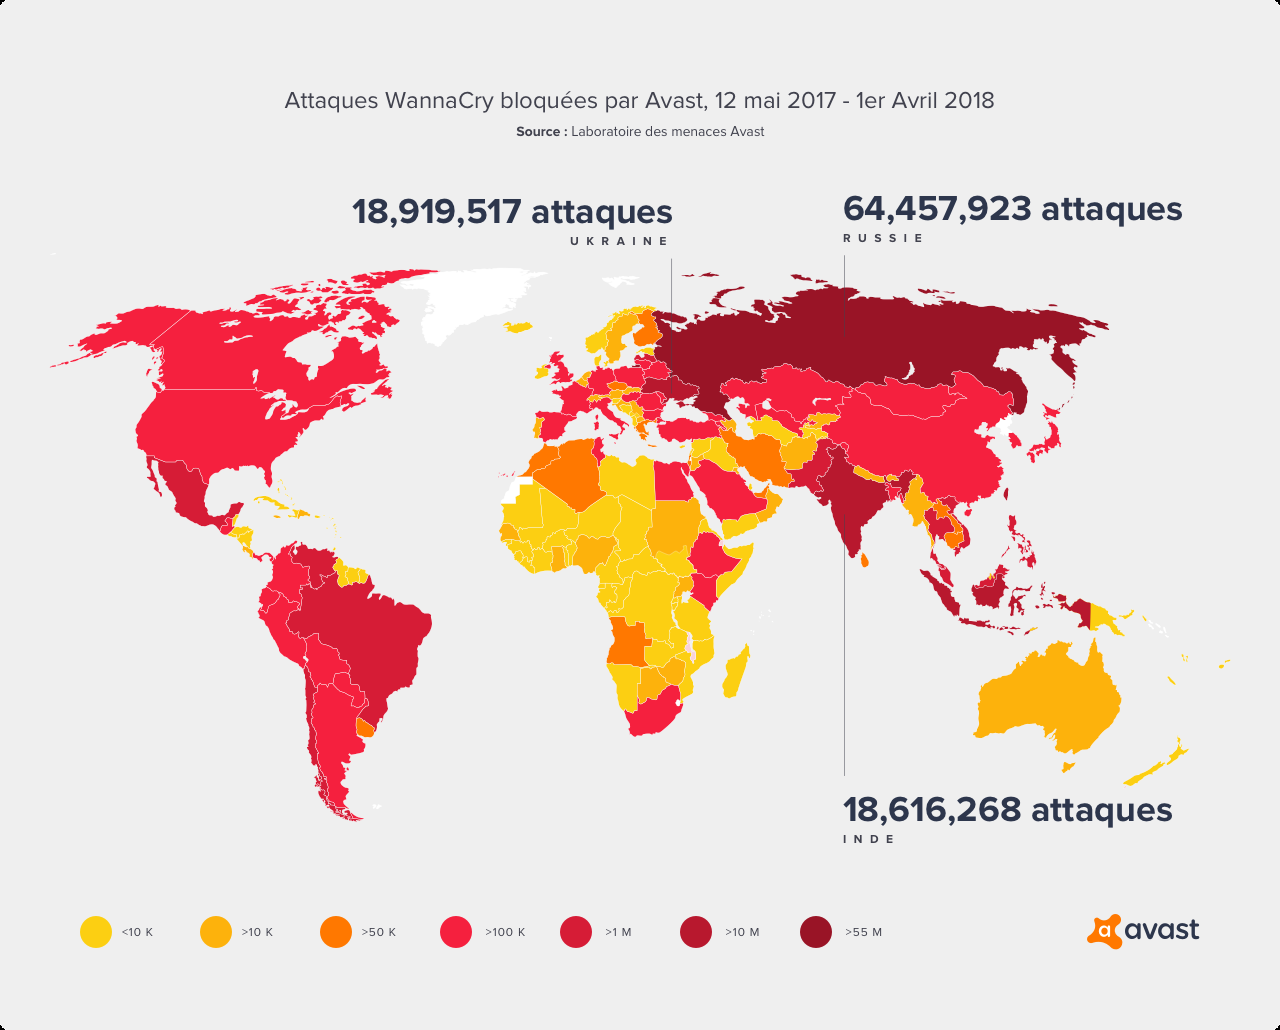
\includegraphics[width=0.85\textwidth]{figures_externes/avast_wannacry_2018_carte.png}
\caption{Tentatives d'attaque {WannaCry} bloquées par pays, $12$~mai $2017$ au $1$er~avril
$2018$. L'échelle logarithmique de la légende (de moins de $10\,000$ à plus de $55$~millions)
donne la mesure de la dispersion entre pays.}
\label{fig:wannacry}
\end{figure}

\paragraph{NotPetya, $2017$ : la propagation.} Un logiciel destructeur diffusé par la mise à jour
d'un logiciel comptable ukrainien s'est propagé aux réseaux de groupes internationaux et en a
paralysé l'activité pendant plusieurs semaines. L'incident naît chez un prestataire (P4), se
propage faute de cloisonnement et de gouvernance des accès (P1), et met à l'épreuve la gestion de
crise (P2). Son traitement assurantiel a en outre donné lieu à des contentieux sur l'exclusion de
guerre des contrats, ce qui rappelle qu'un sinistre cyber peut être avéré sans être couvert.

\paragraph{MOVEit, $2023$ : l'accumulation.} Une vulnérabilité d'un logiciel de transfert de
fichiers, exploitée par un groupe criminel, a permis de dérober des données chez des milliers
d'organisations, souvent atteintes à travers leurs propres prestataires. C'est un choc de cause
commune à l'état pur : une seule défaillance tierce produit de nombreux sinistres simultanés. Le
mémoire l'utilise comme expérience naturelle au chapitre~\ref{ch:identifiabilite}.

\paragraph{CrowdStrike, $2024$ : la dépendance sans adversaire.} Une mise à jour défectueuse d'un
logiciel de sécurité a bloqué des millions de postes de travail dans le transport aérien, la
banque et la santé. Aucune attaque n'est en cause : l'incident relève de la dépendance à un
prestataire (P4) et de l'absence de tests progressifs avant déploiement (P3). Il entre pleinement
dans le champ de DORA, et il montre qu'un périmètre restreint aux seules attaques manquerait une
part substantielle du risque que le règlement vise.

\medskip
\noindent Ces trois cas ont une structure commune : un incident naît sur un domaine de contrôle
et en dégrade d'autres, dans un ordre. Aucune mesure de dépendance symétrique ne restitue cette
structure.

%======================================================================
\section{Pourquoi le risque cyber est difficile à assurer et à capitaliser}
\label{sec:assurabilite-capital}

\subsection{Fréquence, sévérité et contrat d'assurance}
\label{subsec:frequence-severite-contrat}
% HARNAIS-HORS-SECTION: section de cadrage actuariel, aucune valeur chiffree du projet.

La charge annuelle d'un risque se décompose classiquement en un nombre d'événements et un coût
par événement, la fréquence et la sévérité. Cette décomposition n'est pas une commodité de
présentation : elle sépare deux mécanismes que les mêmes mesures ne réduisent pas. Une
sensibilisation des collaborateurs agit sur la fréquence, une capacité de reprise agit sur la
sévérité, et un ratio agrégé qui mélange les deux ne dit pas laquelle est à l'\oe uvre. Le
mémoire applique cette discipline jusqu'au bout, en décomposant l'écart de capital entre états de
conformité plutôt qu'en l'annonçant en niveau global (chapitre~\ref{chap:resultats}).

Le contrat d'assurance introduit deux transformations qu'il faut avoir en tête avant toute
comparaison de montants. La \emph{franchise} laisse à la charge de l'assuré la première tranche
du sinistre ; la \emph{capacité} plafonne l'engagement de l'assureur. Ce que l'assureur verse
n'est donc ni la perte subie ni une fraction fixe de celle-ci, mais une perte subie transformée
par ces deux paramètres, qui varient d'un contrat à l'autre et d'un exercice à l'autre. Une
charge indemnisée et une perte brute ne se comparent ni en niveau ni en quantile.

\paragraph{Cette transformation crée une ambiguïté d'interprétation.} Sur des données agrégées,
une baisse de franchise et une aggravation réelle de la menace produisent le même signal, une
charge indemnisée qui monte. Deux mécanismes, une seule observable, et rien dans la donnée pour
les séparer. C'est, à l'échelle du marché, la situation exacte que le
chapitre~\ref{ch:identifiabilite} rencontre à l'échelle des domaines de contrôle, et le
traitement retenu y est le même : borner plutôt que poser.

\subsection{Dépendance, accumulation et risque systémique}
\label{subsec:dependance-accumulation}
% HARNAIS-HORS-SECTION: section de cadrage, aucune valeur chiffree du projet.

L'assurabilité d'un risque suppose plusieurs conditions, et le cyber les met toutes en tension.
La \emph{mutualisation} suppose des sinistres suffisamment indépendants : la défaillance tierce
la met en défaut par construction. L'\emph{aléa} suppose une survenance non contrôlée par un
tiers intéressé : une attaque ciblée le contredit. La \emph{quantification} suppose un
historique suffisant, dont la sous-section suivante montre l'absence là où elle compte.
L'\emph{aléa moral} et l'\emph{anti-sélection} sont enfin renforcés par l'asymétrie
d'information entre l'assureur et l'assuré sur l'état réel du système d'information de ce
dernier.

Ce dernier point mérite d'être retenu, car c'est celui sur lequel la réglementation agit. DORA
réduit l'asymétrie : il impose un registre des accords avec les prestataires, une notification
des incidents majeurs et des tests de résilience, c'est-à-dire un ensemble d'informations
observables sur la maîtrise du risque. Une méthode qui traduit ce niveau de maîtrise en capital
utilise donc une information que le règlement rend disponible, et qui ne l'était pas avant lui.

\subsection{Rareté des données extrêmes et limite de l'historique français}
\label{subsec:donnees-extremes}
% HARNAIS-HORS-SCRIPT: le niveau reglementaire 99,5 % est pose par la directive ; le recul
% de 20 % des sinistres et les millesimes 2020-2022 viennent d'analyses de sinistralite
% europeennes citees en bibliographie, que le depot ne detient pas et ne recalcule pas.

Le capital de solvabilité se mesure par un \emph{quantile} à $99{,}5\,\%$ de la charge annuelle,
c'est-à-dire par le montant qui n'est dépassé qu'une année sur deux cents. Il se joue donc
entièrement dans les sinistres les plus lourds, et non dans les sinistres courants. Or la donnée
française y est presque vide, ce que la section~\ref{sec:marche-cyber-francais} établit en
chiffres.

La conséquence est méthodologique et elle engage tout le mémoire. La méthode usuelle d'estimation
d'une queue de distribution, dite \emph{par dépassement de seuil}, ne retient que les pertes
au-dessus d'un montant élevé et ajuste une loi sur ces seules observations. Elle exige donc un
effectif suffisant au-dessus du seuil, et l'historique national n'en offre aucun : il s'arrête
avant le haut de la distribution, là précisément où se joue le quantile recherché. Une estimation
conduite sur cette base serait instable d'un exercice à l'autre et sous-estimerait le risque,
faute d'avoir observé les pertes qui le portent. C'est le motif, repris au
chapitre~\ref{chap:donnees}, de calibrer la sévérité sur une base internationale.

Cette rareté ne traduit pas une protection particulière du marché français : les analyses de
sinistres européennes relèvent un recul d'environ $20\,\%$ des sinistres cyber en $2024$ qui
laisse le niveau près d'un tiers au-dessus des exercices $2020$ à $2022$ \citep{marsh2025}, et le
marché britannique voisin est décrit comme plus développé et plus exposé aux sinistres sévères
\citep{dsit2025}.

%======================================================================
\section{Le marché français : diffusion de la couverture et fragilités techniques}
\label{sec:marche-cyber-francais}

\subsection{Le portefeuille LUCY : périmètre et précautions d'interprétation}
\label{subsec:lucy-perimetre}
% SOURCES-SCRIPTS: 63

L'étude LUCY de l'AMRAE, dont l'édition $2026$ porte sur l'exercice $2025$, observe le marché
français à partir de $20\,996$ polices et $1\,251$ sinistres déclarés, recueillis auprès de douze
courtiers et d'un assureur \citep{amraeLucy2026}. La série est engagée depuis $2019$, ce qui donne
sept exercices comparables et permet de distinguer un régime d'un accident d'exercice. L'auteur de
ce mémoire a co-écrit, avec son tuteur, l'analyse actuarielle de cette édition publiée par
Nexialog Consulting \citep{RapiorKaddouri2026}.

Cette source est employée sous un statut précis, celui de \emph{citation externe non
recalculable} : ses valeurs sont reprises telles qu'elle les publie, sans que le mémoire soit en
mesure de les recalculer depuis la donnée d'origine, qui ne lui appartient pas. Aucune n'entre
donc dans un calcul du modèle et aucune ne porte un montant de capital. Ce qui est vérifiable
l'est néanmoins : les valeurs sont recopiées dans un script du dépôt, qui contrôle que le rapport
des sinistres aux primes redonne bien la série des ratios publiée, que la somme des classes de
taille redonne la charge annuelle sur les sept exercices, et que chaque multiplicateur cité se
retrouve à partir des niveaux qui l'encadrent. Ces contrôles portent sur la fidélité de la
recopie, non sur la collecte ni sur le périmètre de l'étude citée, qui relèvent de celle-ci.

\begin{attention}
\textbf{Ces montants ne se comparent pas à ceux du mémoire.} La charge citée dans cette section
est une charge \emph{indemnisée}, donc nette de franchise et plafonnée par la capacité, au sens
de la sous-section~\ref{subsec:frequence-severite-contrat}. Elle vaut $83{,}2$~M\euro{} en $2025$
contre $54{,}5$ l'exercice précédent, soit une hausse de $53\,\%$. La sévérité que le présent
mémoire modélise est d'une tout autre nature : c'est la perte \emph{brute} subie par une entité
financière, avant toute assurance. Les rapprocher conduirait à lire un écart de définition comme
une contradiction.
\end{attention}

\subsection{Soft market, baisse des prix et dégradation de la sinistralité}
\label{subsec:lucy-soft-market}
% SOURCES-SCRIPTS: 63

Entre $2024$ et $2025$, le nombre d'entreprises assurées croît de $49\,\%$ quand les primes
souscrites reculent de $3\,\%$, et le ratio sinistres sur primes remonte pour le troisième
exercice, de $12\,\%$ en $2023$ à $27\,\%$ en $2025$, loin toutefois des $169\,\%$ de $2020$. Le
marché se diffuse donc par le volume et non par le budget : davantage d'entreprises sont
couvertes, pour une prime moyenne plus faible, au moment même où la sinistralité remonte.

\begin{figure}[htbp]
\centering
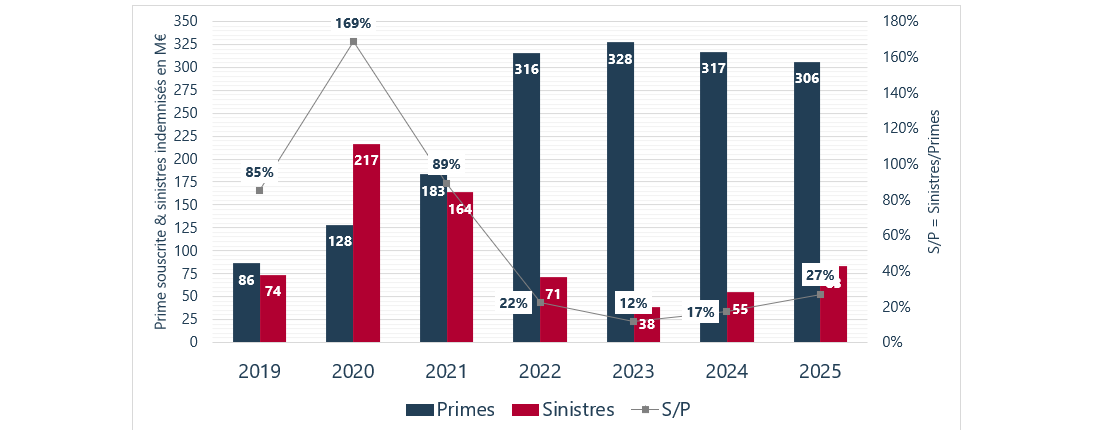
\includegraphics[width=0.85\textwidth]{figures_externes/lucy_primes_sinistres_ratio.png}
\caption{Primes souscrites, sinistres indemnisés et ratio sinistres sur primes, $2019$--$2025$.
La sinistralité remonte pour le troisième exercice consécutif alors que les primes reculent.}
\label{fig:lucy-ratio}
\end{figure}

Cette configuration est instable par construction, et c'est ce qui donne un intérêt opérationnel
à une mesure du risque indépendante du cycle tarifaire. Le recul du taux de prime atteint
$33\,\%$ sur les grandes entreprises et $23\,\%$ sur les entreprises de taille intermédiaire :
l'assouplissement est réel, mais il ne repose sur aucune amélioration mesurée de la maîtrise du
risque.

\subsection{Deux régimes de sinistralité : sévérité en 2024, fréquence en 2025}
\label{subsec:lucy-freq-sev}
% SOURCES-SCRIPTS: 63

L'indicateur suivi par le marché est le ratio sinistres sur primes, c'est-à-dire la part de la
prime qui part en indemnisation. Il a monté deux exercices de suite, mais pour deux raisons
opposées, et seule sa décomposition le montre. La charge d'une année se met en effet sous la
forme d'un produit de deux termes, le \emph{nombre} de sinistres survenus et le \emph{sinistre
moyen}. Le tableau compare chaque terme à sa valeur de l'année précédente, sous la forme d'un
multiplicateur.

\begin{center}\small
\renewcommand{\arraystretch}{1.2}
\begin{tabular}{@{}l r r r l@{}}
\toprule
& \textbf{nombre} & \textbf{sinistre moyen} & \textbf{charge} & \textbf{régime} \\
\midrule
Marché, exercice $2024$ & $\times 0{,}73$ & $\times 1{,}96$ & $\times 1{,}43$ & sévérité \\
Marché, exercice $2025$ & $\times 2{,}79$ & $\times 0{,}55$ & $\times 1{,}53$ & fréquence \\
\midrule
\multicolumn{5}{@{}l}{\emph{Exercice $2025$, par bloc}} \\
grandes entreprises & $\times 1{,}24$ & $\times 0{,}82$ & $\times 1{,}02$ & absorbé \\
bloc intermédiaire & $\times 2{,}14$ & $\times 1{,}65$ & $\times 3{,}53$ & les deux \\
micro-entreprises & $\times 9{,}52$ & $\times 0{,}73$ & $\times 6{,}97$ & nombre seul \\
\bottomrule
\end{tabular}
\end{center}

\vspace{2pt}
\noindent En $2024$ le nombre de sinistres a baissé alors que leur coût moyen a doublé : la charge
a monté parce que les sinistres étaient plus lourds. En $2025$ c'est l'inverse, le coût moyen a
baissé de moitié alors que le nombre a presque triplé. Le ratio seul ne permet pas de distinguer
ces deux situations, qui n'appellent pourtant pas les mêmes mesures. Le bloc intermédiaire est le
seul segment où le nombre et le coût moyen augmentent en même temps, ce qui explique sa charge
multipliée par $3{,}53$.

\noindent Ces multiplicateurs portent sur le \emph{nombre} de sinistres, un total, et non sur la
\emph{fréquence}, qui le rapporte au nombre d'assurés : l'égalité charge $=$ nombre $\times$ coût
moyen n'est exacte qu'avec le nombre.

\subsection{Polarisation du marché et limites de la donnée assurantielle}
\label{subsec:lucy-polarisation}
% SOURCES-SCRIPTS: 63

La divergence entre le prix et le risque ne se répartit pas uniformément. Le segment dont la
sinistralité progresse le plus n'est pas celui dont le tarif se redresse, et les multiplicateurs
les plus spectaculaires portent sur les micro-entreprises, dont la part dans la charge totale
reste marginale. Un multiplicateur hiérarchise des dynamiques, jamais des enjeux.

\begin{figure}[htbp]
\centering
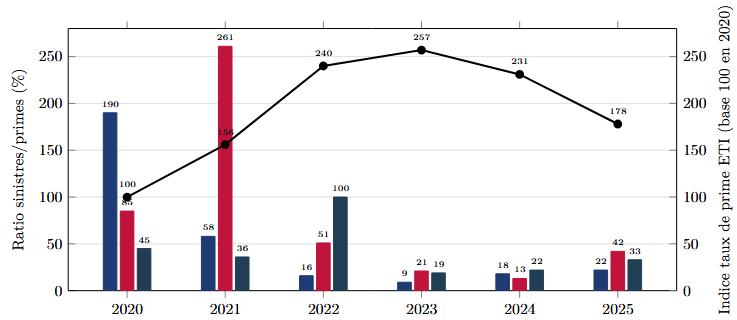
\includegraphics[width=0.85\textwidth]{figures_externes/lucy_divergence_prix_risque.png}
\caption{Divergence entre le prix et le risque par segment. Le segment dont la sinistralité
progresse le plus n'est pas celui dont le tarif se redresse.}
\label{fig:lucy-divergence}
\end{figure}

\paragraph{La limite qui engage le mémoire est ailleurs, et elle est dans la queue.} Deux
exercices sur sept ne portent aucun sinistre de la classe de taille la plus haute ; un exercice
en porte $135$~M\euro{} et l'exercice sous revue $19$~M\euro, pour un seul sinistre dépassant
$10$~M\euro. Le maximum de la série vaut $7{,}11$ fois le montant de l'exercice sous revue, ce qui
donne la mesure de l'irrégularité.

\begin{figure}[htbp]
\centering
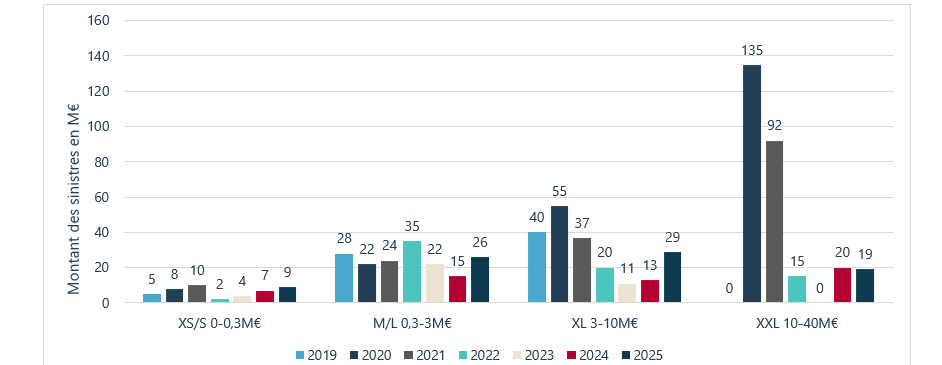
\includegraphics[width=0.85\textwidth]{figures_externes/lucy_taille_des_sinistres.png}
\caption{Charge indemnisée par classe de taille de sinistre, $2019$--$2025$. La classe la plus
haute est vide deux exercices sur sept : l'historique national s'arrête avant le haut de la
distribution.}
\label{fig:lucy-taille}
\end{figure}

C'est la mesure annoncée à la sous-section~\ref{subsec:donnees-extremes}, et elle tranche le
choix de la base de calibration.

%======================================================================
\section{DORA : de la résilience opérationnelle à la maîtrise des dépendances}
\label{sec:dora}
% HARNAIS-HORS-SECTION: section reglementaire. Les seuls nombres sont des millesimes, des
% numeros d'articles et des references de textes, aucun ne provient d'un calcul du projet.

\subsection{Le cadre réglementaire européen du cyber}
\label{subsec:cadre-reglementaire-europeen}
% HARNAIS-HORS-SECTION: section reglementaire, les seuls nombres sont la date d'entree en
% application du reglement et des millesimes de textes.

Le cadre européen s'est construit par strates. La directive sur la sécurité des réseaux et des
systèmes d'information a posé des exigences minimales de sécurité et de notification pour les
opérateurs de services essentiels, puis sa refonte en a élargi le périmètre et renforcé les
obligations de gouvernance. Le règlement général sur la protection des données a fixé, en
parallèle, un régime de notification et de sanction propre aux données personnelles. Ces deux
textes portent sur la sécurité et sur la confidentialité, non sur la continuité d'une activité
financière.

C'est ce que le règlement sur la résilience opérationnelle numérique du secteur financier, dit
DORA, vient combler. Entré en application le $17$ janvier $2025$, il s'adresse à une vingtaine de
catégories d'entités financières, dont les entreprises d'assurance, et il déplace l'objectif :
il ne s'agit plus seulement d'empêcher l'incident mais de garantir que l'entité \emph{résiste,
réagit et se rétablit} lorsqu'il survient. Cette bascule est celle qui rend le sujet actuariel,
car un objectif de continuité se mesure en pertes évitées et en durées d'indisponibilité, donc
en grandeurs que l'on peut chiffrer.

\subsection{Les cinq piliers de DORA}
\label{subsec:cinq-piliers-dora}
% HARNAIS-HORS-SECTION: section reglementaire, les seuls nombres sont les etiquettes P1 a P5
% des cinq piliers.

Le règlement organise la résilience autour de cinq domaines, que le mémoire note P1 à P5 et
traite comme des domaines de \emph{contrôle} plutôt que comme des obligations à cocher.

\begin{itemize}[leftmargin=1.4em,itemsep=4pt]
\item \textbf{P1, gouvernance du risque lié aux technologies.} L'organe de direction est
      explicitement responsable du dispositif, et cette responsabilité n'est pas délégable :
      stratégie de résilience, cartographie des actifs informationnels et des dépendances
      critiques, politique de sécurité documentée, et contrôle interne continu plutôt
      qu'audits ponctuels.
\item \textbf{P2, gestion, classification et notification des incidents.} Détection,
      qualification selon des critères de matérialité, puis notification des incidents
      \emph{majeurs} selon un calendrier resserré : alerte sous quatre heures après
      classification et au plus tard vingt-quatre heures après détection, rapport
      intermédiaire sous soixante-douze heures, rapport final sous un mois.
\item \textbf{P3, tests de résilience opérationnelle numérique.} Les procédures ne se
      documentent plus, elles s'éprouvent. Les entités identifiées comme significatives sont
      soumises à des tests de pénétration guidés par la menace, à mener au moins tous les
      trois ans en conditions proches du réel.
\item \textbf{P4, gestion du risque lié aux prestataires tiers.} Recensement des contrats
      critiques dans un registre d'informations harmonisé, clauses contractuelles impératives,
      stratégie de sortie, et surveillance directe des prestataires tiers jugés critiques par
      les autorités européennes, jusqu'au troisième rang de la chaîne de sous-traitance.
\item \textbf{P5, partage d'informations sur les cybermenaces.} Échange, sur une base
      volontaire et encadrée, de renseignements entre entités financières. C'est le pilier le
      moins mobilisable dans un calibrage actuariel, et il rappelle que la résilience porte
      une dimension collective au-delà de l'entité.
\end{itemize}

\paragraph{La lecture que le mémoire en fait.} Ces cinq domaines ne sont pas indépendants, et
c'est l'hypothèse de travail de tout le document. La défaillance de l'un dégrade la capacité de
l'entité à tenir les autres, selon le mécanisme décrit à la
sous-section~\ref{subsec:chocs-cause-commune} et formalisé au chapitre~\ref{chap:cascade}. La
non-conformité ne reste pas dans son pilier.

\subsection{Prestataires TIC, concentration et propagation du risque}
\label{subsec:risque-tiers-dora}
% HARNAIS-HORS-SECTION: section reglementaire, aucune valeur chiffree.

Le quatrième pilier est celui qui a motivé le règlement autant que les autres réunis. La chaîne
de sous-traitance informatique du secteur financier est concentrée sur un petit nombre de
fournisseurs d'infrastructure, de logiciels de gestion et de services de sécurité, si bien qu'une
défaillance chez l'un d'eux atteint simultanément de nombreuses entités sans qu'aucune n'ait
commis de faute. C'est la raison pour laquelle DORA ne se contente pas d'exiger des clauses
contractuelles : il instaure un cadre de surveillance directe des prestataires désignés comme
critiques, ce qui est une nouveauté dans l'architecture prudentielle européenne.

Cette concentration n'est pas une conjecture : la sous-section~\ref{subsec:france-assureurs-cesin}
la mesure, en montrant que l'attaque indirecte par un tiers est le vecteur dont la part croît le
plus nettement avec la taille de l'entité.

\paragraph{Le registre d'informations pèse plus que les autres exigences pour la modélisation.}
En imposant le recensement exhaustif des contrats TIC critiques et de leurs chaînes de
sous-traitance, le règlement produit une donnée exploitable pour modéliser le risque de
concentration technologique. Cette donnée faisait défaut à l'évaluation interne des risques
traditionnelle, qui décrivait la dépendance sans pouvoir la chiffrer. C'est le point de contact
le plus direct entre une obligation réglementaire et une entrée de modèle, et le
chapitre~\ref{ch:robustesse} y revient pour dire ce que le registre ne donnera pas non plus.

\subsection{Les autorités françaises et la supervision de la résilience numérique}
\label{subsec:supervision-france}
% HARNAIS-HORS-SECTION: section institutionnelle, aucune valeur chiffree.

La supervision se répartit entre plusieurs autorités aux compétences distinctes. L'Autorité de
contrôle prudentiel et de résolution supervise les entreprises d'assurance et intègre le risque
informatique à sa démarche prudentielle ; l'Autorité des marchés financiers encadre les sociétés
de gestion ; l'Agence nationale de la sécurité des systèmes d'information porte la prévention et
la réponse aux incidents affectant les systèmes critiques ; et la Commission nationale de
l'informatique et des libertés veille au respect du régime des données personnelles. Au niveau
européen, les trois autorités de surveillance sectorielles coordonnent la désignation et la
surveillance des prestataires tiers critiques.

Cette répartition a une conséquence pour le mémoire : aucune de ces autorités ne publie de
probabilité de propagation entre domaines de contrôle. Elles publient des attentes prudentielles
et des échelles de maturité, ce qui n'est pas la même chose. C'est le motif pour lequel les
valeurs de propagation du modèle sont posées à dire d'expert puis bornées, et non présentées
comme calibrées sur une source officielle.

%======================================================================
\section{Un risque prioritaire sans traduction prudentielle directe}
\label{sec:enjeu-prudentiel}

\subsection{La perception prospective : France Assureurs et CESIN}
\label{subsec:france-assureurs-cesin}
% SOURCES-SCRIPTS: 103 63

Deux sources annuelles, de nature différente, situent le risque cyber. La cartographie
prospective de la profession classe les risques selon leur fréquence et leur gravité anticipées
\citep{franceassureurs2026} ; le baromètre mené auprès des responsables de la sécurité des
systèmes d'information recense les vecteurs et les conséquences \emph{déclarés}
\citep{cesin2026}. La première mesure une anticipation, la seconde un constat.

\paragraph{Le risque cyber sature au sommet de la cartographie.} Il occupe la première place pour
le huitième exercice consécutif, avec un score moyen de $4{,}1$ sur $5$, devant l'environnement
économique à $4{,}0$ et le dérèglement climatique à $3{,}9$. Mais son score ne monte plus : il
culmine à $4{,}48$ lors de l'édition $2022$ et redescend à $4{,}10$ en $2026$. Une préoccupation
installée au sommet d'un classement cesse d'être informative par son rang, et le renseignement
passe dans la manière dont elle se déforme.

\begin{figure}[htbp]
\centering
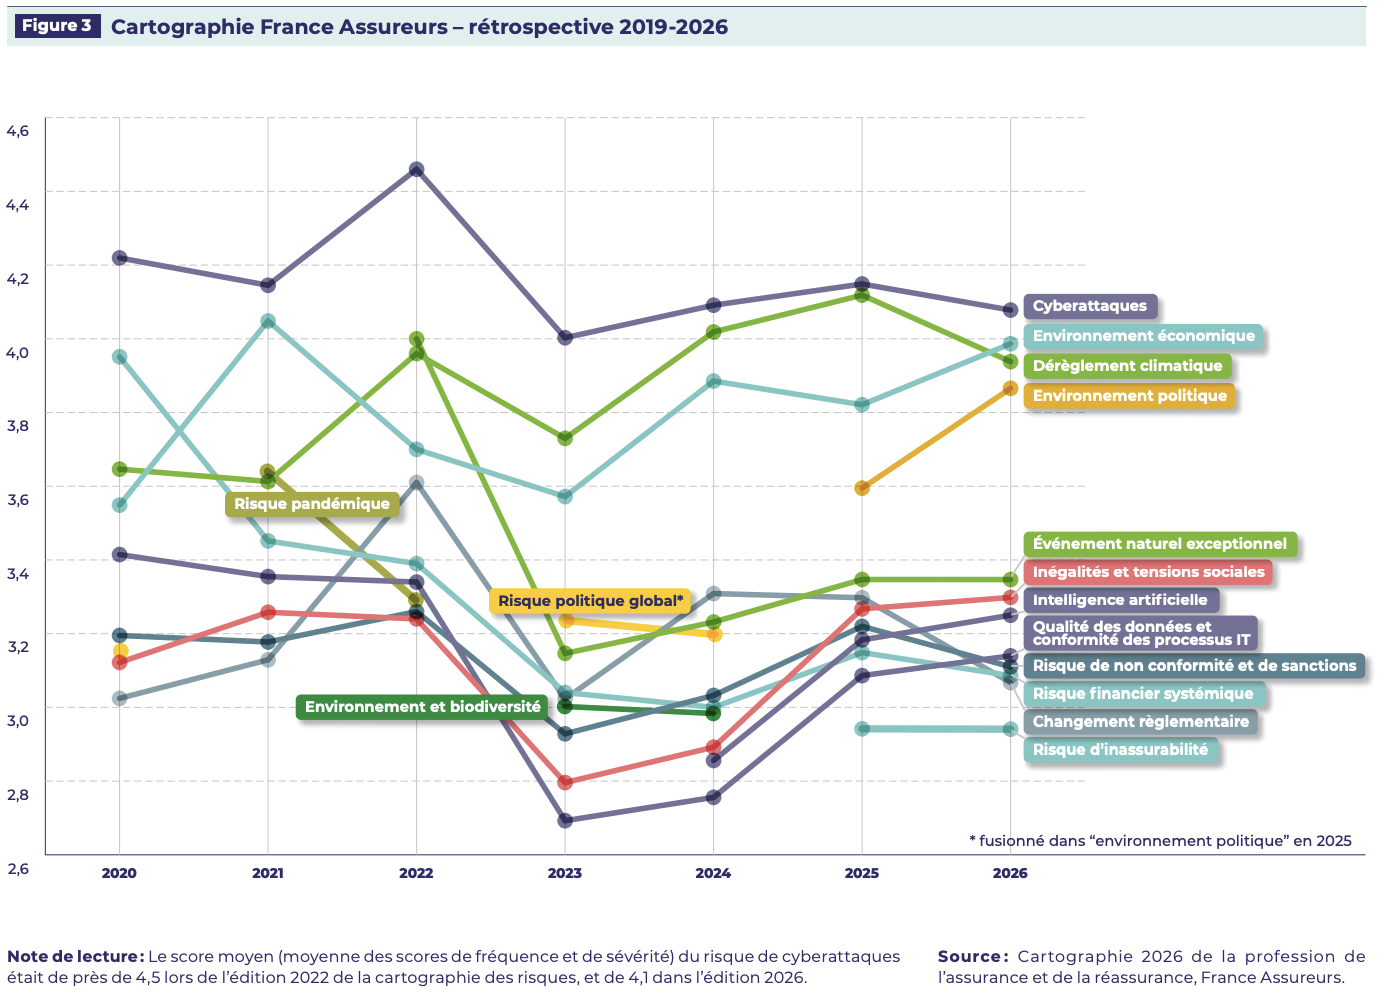
\includegraphics[width=0.92\textwidth]{figures_externes/carto_fa_2026_retrospective.png}
\caption{Trajectoire des scores de la cartographie prospective, $2020$--$2026$. Le risque de
cyberattaques reste au premier rang mais son score a cessé de monter depuis $2022$.}
\label{fig:carto-retro}
\end{figure}

\paragraph{Et la déformation est un changement de régime.} Entre $2025$ et $2026$, le risque de
cyberattaques recule de $0{,}45$ point en fréquence anticipée et progresse de $0{,}25$ point en
sévérité : moins d'événements attendus, mais plus lourds. Le risque qui progresse le plus en
sévérité sur cette édition n'est d'ailleurs pas le cyber mais la qualité des données et la
conformité des processus informatiques, à $+0{,}30$ point, et la cartographie fait désormais
figurer un risque de non-conformité et de sanctions ainsi qu'un risque lié à l'intelligence
artificielle. La préoccupation de la profession se déplace de la menace vers sa
\emph{gouvernance}, ce qui est l'objet même de DORA.

\paragraph{Le baromètre confirme le recul de fréquence et nomme le vecteur qui compte.} Sur
l'exercice $2025$, $40\,\%$ des entreprises interrogées déclarent avoir subi au moins une
cyberattaque significative. Parmi les $159$ qui en ont constaté une, l'hameçonnage domine à
$55\,\%$, devant l'exploitation d'une faille à $41\,\%$. Chaque entreprise attaquée cite en
moyenne $3{,}3$ vecteurs, contre $4{,}0$ à la vague précédente : une attaque n'emprunte presque
jamais un chemin unique.

\begin{figure}[htbp]
\centering
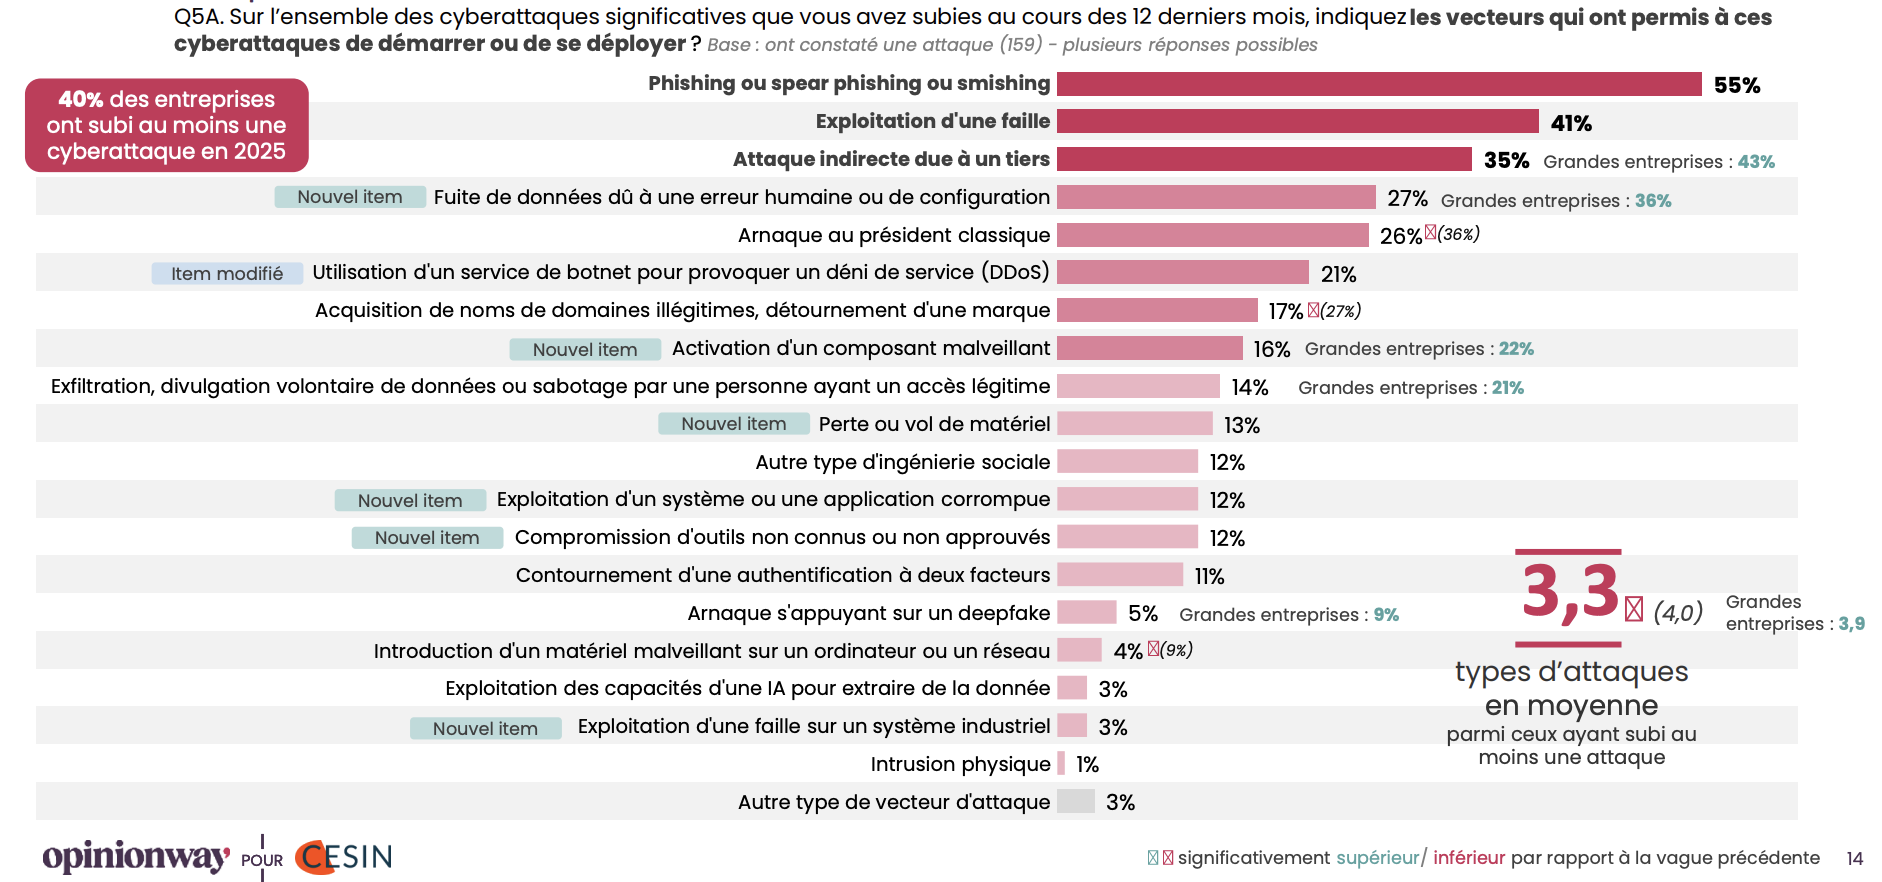
\includegraphics[width=0.80\textwidth]{figures_externes/cesin_2026_vecteurs.png}
\caption{Vecteurs ayant permis aux cyberattaques de démarrer ou de se déployer, exercice $2025$.
Les mentions de droite donnent la part chez les grandes entreprises là où elle diffère
significativement de la moyenne.}
\label{fig:cesin-vecteurs}
\end{figure}

Le troisième vecteur est celui que le mémoire modélise. L'attaque indirecte par un tiers pèse
$35\,\%$, et sa part monte à $43\,\%$ chez les grandes entreprises. Plus une entité est grande,
plus son exposition passe par ses prestataires : c'est le domaine P4, mesuré de l'extérieur par
une source sans lien avec ce travail. Les trois autres vecteurs dont la part croît avec la
taille, la fuite par erreur de configuration à $36\,\%$, l'activation d'un composant malveillant
à $22\,\%$ et l'exfiltration par un accès légitime à $21\,\%$, relèvent tous de la gouvernance des
accès, c'est-à-dire du domaine P1. Les vecteurs qui montent avec la taille sont donc ceux qui
passent par un tiers ou par un accès autorisé, non ceux qui forcent un périmètre.

\paragraph{Les conséquences, et celle qu'il faut isoler.} Quatre entreprises attaquées sur cinq
déclarent un impact sur leur activité, soit $81\,\%$ contre $19\,\%$ sans impact. Les
conséquences dominantes sont la perturbation de la production à $28\,\%$ et la perte d'image à
$26\,\%$, devant la compromission de savoir-faire et la perte de chiffre d'affaires à $18\,\%$
chacune. La sanction d'une autorité ne concerne que $3\,\%$ des cas : le canal réglementaire est
réel mais minoritaire, et un modèle qui ferait de l'amende le principal coût de la non-conformité
se tromperait de mécanisme.

Une conséquence mérite d'être isolée. La déconnexion par les tiers, c'est-à-dire la mise en
quarantaine de l'entité par ses propres partenaires, est citée dans $12\,\%$ des cas. Elle
renverse le constat précédent : une entité n'est pas seulement atteinte \emph{par} ses
partenaires, elle est aussi coupée \emph{par} eux lorsqu'elle est atteinte. La dépendance joue
dans les deux sens, et les deux sens n'ont ni le même coût ni la même prévention. Aucune mesure
de dépendance symétrique ne peut les distinguer.

\begin{attention}
\textbf{Deux sources qui semblent se contredire, et ne se contredisent pas.} Le baromètre et la
cartographie décrivent un recul de la fréquence, quand le marché assuré affiche un nombre de
sinistres presque triplé (sous-section~\ref{subsec:lucy-freq-sev}). Les deux constats sont
compatibles : le nombre de sinistres du marché est un \emph{total}, porté par une base d'assurés
élargie de $49\,\%$ sur le même exercice, alors que les deux autres sources mesurent une
exposition \emph{par entité}. Un marché peut enregistrer davantage de sinistres tout en assurant
des entités individuellement moins exposées. Confondre le total et la fréquence conduirait à lire
une aggravation là où il y a une extension de périmètre. Ces deux enquêtes sont par ailleurs
déclaratives : elles mesurent ce que les organisations constatent, non ce qui survient.
\end{attention}

\subsection{Les limites de Solvabilité II et de la Formule Standard}
\label{subsec:limites-formule-standard}
% HARNAIS-HORS-SECTION: section de cadrage prudentiel, aucune valeur chiffree du projet.

Le risque cyber est donc au premier rang des préoccupations, mesuré par plusieurs sources
indépendantes, et encadré depuis $2025$ par un règlement qui en rend la maîtrise observable.
Aucun dispositif prudentiel ne traduit pourtant ce niveau de maîtrise en capital.

La Formule Standard de Solvabilité~II charge le risque opérationnel par un pourcentage de primes
ou de provisions techniques. Ce forfait est \emph{plat} en conformité : deux entités de bilan
identique et de maturité opposée sur les cinq domaines de DORA acquittent exactement la même
charge. Aucun sous-module cyber n'existe, et le risque couvert par les garanties affirmatives ne
correspond à aucun module standard, ce qui renvoie les assureurs à leurs modèles internes et à
leur évaluation interne des risques et de la solvabilité. L'articulation juridique complète entre
les deux textes est traitée au chapitre~\ref{chap:reglementaire}.

Les outils actuariels usuels ne comblent pas ce vide. Une copule capturerait la co-occurrence des
pertes entre domaines de contrôle, mais symétriquement : elle ne distingue pas une défaillance
qui \emph{entraîne} les autres d'une défaillance qui les \emph{subit}. Or c'est cette asymétrie
qui devrait commander la priorité de remédiation. Deux matrices de dépendance transposées l'une
de l'autre, que les statistiques usuelles ne permettent pas de distinguer, conduisent à un
capital et à une décision différents : le chapitre~\ref{chap:cascade} le démontre.

\subsection{Problématique, positionnement et plan du mémoire}
\label{subsec:problematique-positionnement}
% SOURCES-SCRIPTS: 43 68 92

\begin{cle}
\textbf{Question centrale.} Comment traduire un niveau de non-conformité à DORA, même
hypothétique ou graduel, en une distribution de pertes puis en une charge de capital ? Le mémoire
ne pose pas la question \emph{l'entité est-elle conforme aujourd'hui}, mais \emph{combien coûte en
capital de ne pas se conformer}.

\textbf{Ce que désigne le SCR du titre.} Le capital calculé suit la mesure de risque de
Solvabilité~II, un quantile à $99{,}5\,\%$ de la charge annuelle, mais il n'est pas un SCR
réglementaire : aucun module DORA n'existe en Formule Standard. C'est un besoin de capital au
sens de l'évaluation interne des risques, et le corps du mémoire le nomme ainsi.
\end{cle}

Le mémoire s'articule autour de trois apports, et il est aussi explicite sur ce qu'il
\emph{n'affirme pas} que sur ce qu'il établit.

\begin{enumerate}[leftmargin=1.4em,itemsep=3pt]
\item Un mécanisme de dépendance dirigée et sensible à l'ordre entre les piliers, la cascade,
      dont trois propriétés sont démontrées (chapitre~\ref{chap:cascade}) : la criticité dépend
      de l'\emph{ordre} de la chaîne et non du seul ensemble des piliers touchés, ce qu'aucune
      dépendance symétrique ne reproduit ; la normalisation de Leontief borne la propagation ; et
      une matrice et sa transposée, indiscernables pour les statistiques que les sources
      disponibles permettent de construire, donnent un capital et une décision différents.
\item Une frontière d'identifiabilité, démontrée au chapitre~\ref{ch:identifiabilite} puis muée
      en méthode au chapitre~\ref{chap:partielle} : la direction n'étant pas identifiable, le
      mémoire ne la pose pas, il borne le capital sur l'ensemble des matrices admissibles et
      chiffre en euros la valeur de la donnée manquante.
\item Une lecture décisionnelle : le surcoût de non-conformité, son attribution par pilier et
      l'ordre de remédiation, présentés en rapports et en bornes plutôt qu'en niveaux
      (chapitre~\ref{chap:resultats}).
\end{enumerate}

\paragraph{Le fil, en cinq mouvements.} Le mémoire construit d'abord le mécanisme et en démontre
les propriétés (chapitre~\ref{chap:cascade}). Il fait ensuite de la conformité un état qui évolue
et pilote le capital (chapitre~\ref{chap:multietats}). Il délimite alors ce que la donnée permet
d'en estimer (chapitre~\ref{ch:identifiabilite}). Il transforme cette limite en méthode,
l'identification partielle, qui borne le capital plutôt que de poser un paramètre inconnu
(chapitre~\ref{chap:partielle}). Il en tire enfin le surcoût, son attribution, la trajectoire du
capital et l'ordre de remédiation (chapitre~\ref{chap:resultats}).

\begin{cle}
\textbf{Le résultat en bref.} Entre l'état conforme et l'état non conforme sur les quatre canaux
que la conformité déplace, le besoin de capital passe de $6\,049$ à $20\,188$~M\euro{} à
l'échelle du secteur, soit un facteur $3{,}34$ et un écart de $14\,139$~M\euro{}. Ce montant est
un besoin de capital au sens de l'évaluation interne et non un SCR réglementaire : il sert à
comparer deux états, non à remplacer la Formule Standard. Les canaux interagissent, l'interaction
portant $5\,001$~M\euro{}, soit $35\,\%$ de l'écart, et la fréquence seule en produit davantage
qu'aucun autre canal, à $10\,377$~M\euro{} contre $11\,413$ pour les trois autres réunis. Les
niveaux de propagation sont posés, mais la thèse ne dépend que de leur ordre, le besoin de
capital étant croissant en ce paramètre.
\end{cle}

\begin{attention}
\textbf{Ce que le mémoire ne prétend pas.} La matrice de contagion n'est jamais présentée comme
calibrée : elle est posée à dire d'expert et bornée par une analyse de sensibilité. Le niveau
absolu du capital est illustratif, non une mesure : c'est l'effet \emph{relatif} de la conformité
et la hiérarchie des piliers qui sont défendus.
\end{attention}
